%%
%% This is file `sample-sigconf.tex',
%% generated with the docstrip utility.
%%
%% The original source files were:
%%
%% samples.dtx  (with options: `sigconf')
%% 
%% IMPORTANT NOTICE:
%% 
%% For the copyright see the source file.
%% 
%% Any modified versions of this file must be renamed
%% with new filenames distinct from sample-sigconf.tex.
%% 
%% For distribution of the original source see the terms
%% for copying and modification in the file samples.dtx.
%% 
%% This generated file may be distributed as long as the
%% original source files, as listed above, are part of the
%% same distribution. (The sources need not necessarily be
%% in the same archive or directory.)
%%
%% The first command in your LaTeX source must be the \documentclass command.
\documentclass[sigconf]{acmart}
\settopmatter{printacmref=false}
%%
%% \BibTeX command to typeset BibTeX logo in the docs
\AtBeginDocument{%
  \providecommand\BibTeX{{%
    \normalfont B\kern-0.5em{\scshape i\kern-0.25em b}\kern-0.8em\TeX}}}

%% Rights management information.  This information is sent to you
%% when you complete the rights form.  These commands have SAMPLE
%% values in them; it is your responsibility as an author to replace
%% the commands and values with those provided to you when you
%% complete the rights form.
\setcopyright{iw3c2w3}
\copyrightyear{\the\year{}}
\acmYear{\the\year{}}


%%
%% end of the preamble, start of the body of the document source.
\begin{document}

%%
%% The "title" command has an optional parameter,
%% allowing the author to define a "short title" to be used in page headers.
\title{Technologies to support motor skill learning - musical instruments}

%%
%% The "author" command and its associated commands are used to define
%% the authors and their affiliations.
%% Of note is the shared affiliation of the first two authors, and the
%% "authornote" and "authornotemark" commands
%% used to denote shared contribution to the research.
\author{Chaoneng Xie}
%\orcid{1234-5678-9012}
\email{Chaoneng.Xie@campus.lmu.de}
\affiliation{%
  \institution{LMU Munich}
  \city{Munich}
  \country{Germany}
}


%%
%% By default, the full list of authors will be used in the page
%% headers. Often, this list is too long, and will overlap
%% other information printed in the page headers. This command allows
%% the author to define a more concise list
%% of authors' names for this purpose.
%\renewcommand{\shortauthors}{Trovato and Tobin, et al.}

%%
%% The abstract is a short summary of the work to be presented in the
%% article.
\begin{abstract}
  Music education has a tendency to lean towards its tradition, learning of a traditional acoustic instrument such as piano or violin requires observation of established discipline. The standards of a good musical performance and ways of learning and practicing has seldom changed through the years. However, educaters and researchers are always looking for a better way of teaching and practicing. In this digital age, especially after the impact of the pandemic, the innovation of music education is going slowly but continously. New devices and technologies are invented and experimented to provide music learners a better and easier learning experience. In this paper we investigate and review these new technologies. We conducted a literature search using keywords "motor skill", "motor learning", "musical instrument" and "piano" in the following databases: \textit{ACM}, \textit{Springer} and \textit{IEEE Xplore}.\\

  We will classify and compare these different technologies in regarding to supporting the learning of a musical instrument, and evaluate their effektivness. With this result we will try to predict the possible directions of this field of study in the future.\\
\end{abstract}

%%
%% The code below is generated by the tool at http://dl.acm.org/ccs.cfm.
%% Please copy and paste the code instead of the example below.
%%
\begin{CCSXML}
<ccs2012>
   <concept>
       <concept_id>10003120.10003121.10003126</concept_id>
       <concept_desc>Human-centered computing~HCI theory, concepts and models</concept_desc>
       <concept_significance>300</concept_significance>
       </concept>
 </ccs2012>
\end{CCSXML}

\ccsdesc[300]{Human-centered computing~HCI theory, concepts and models}

%%
%% Keywords. The author(s) should pick words that accurately describe
%% the work being presented. Separate the keywords with commas.
\keywords{motor skill, motor learning, musical instrument, piano}

%% A "teaser" image appears between the author and affiliation
%% information and the body of the document, and typically spans the
%% page.
%\begin{teaserfigure}
%  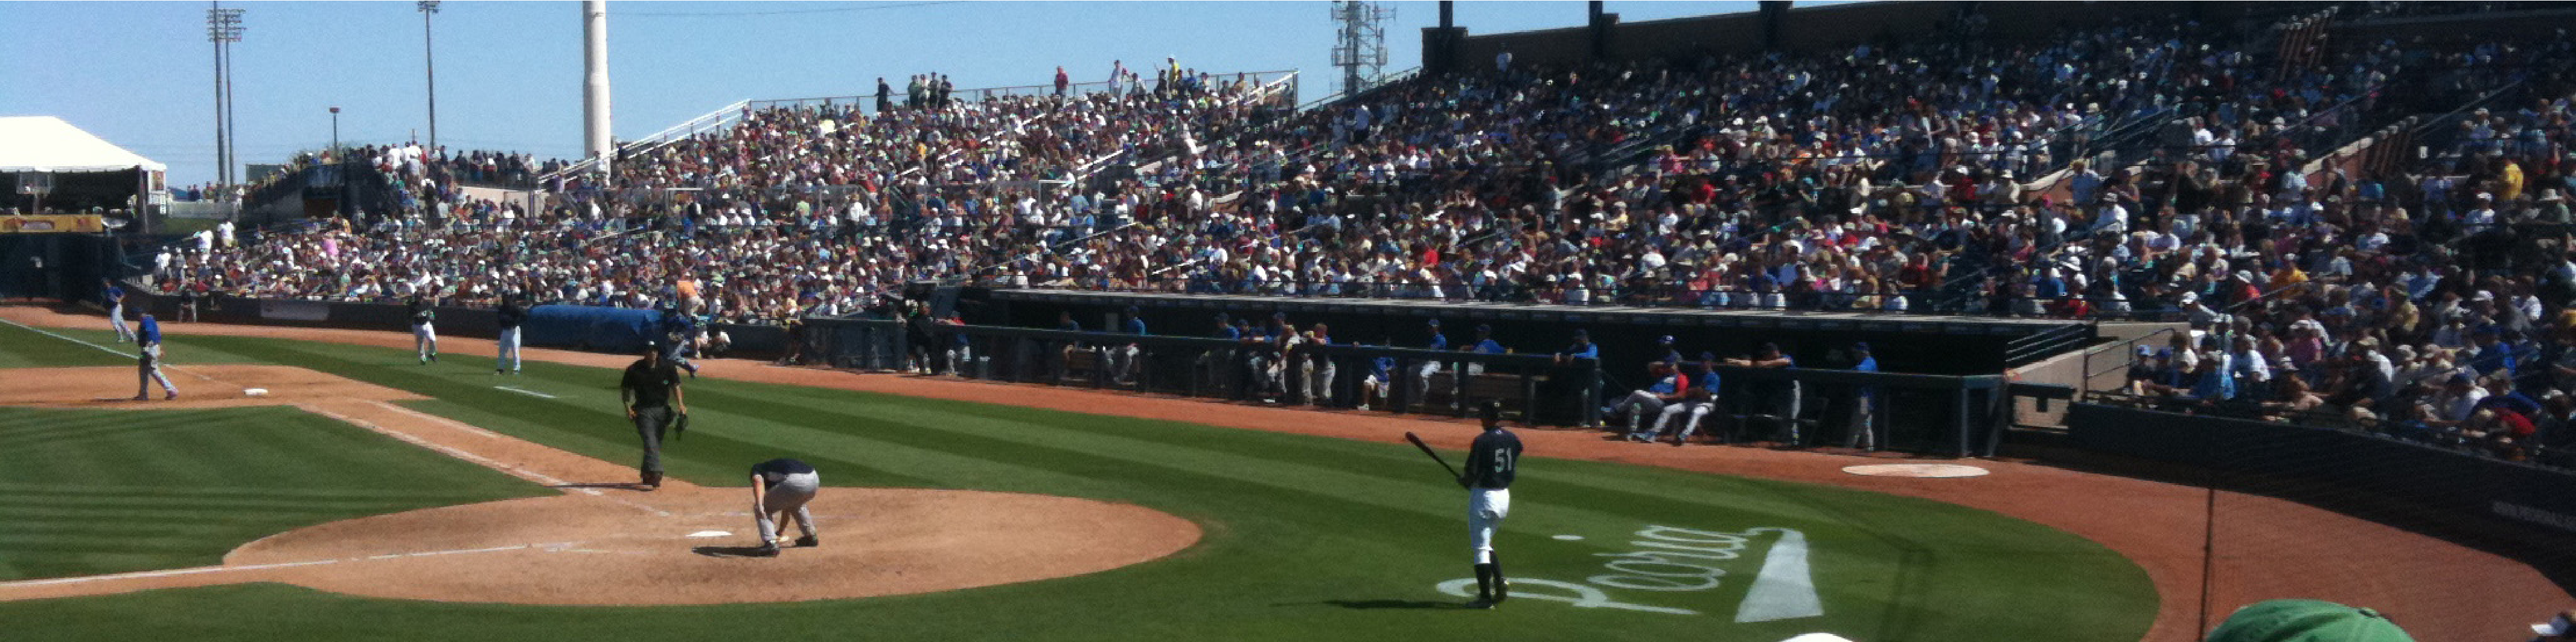
\includegraphics[width=\textwidth]{figures/sampleteaser}
%  \caption{Seattle Mariners at Spring Training, 2010.}
%  \Description{Enjoying the baseball game from the third-base
%  seats. Ichiro Suzuki preparing to bat.}
%  \label{fig:teaser}
%\end{teaserfigure}

%%
%% This command processes the author and affiliation and title
%% information and builds the first part of the formatted document.
\maketitle

\section{Introduction}

\subsection{What is a Good Musical Performance?}
- In the aspekt of traditional music appreciation.\\
- In the aspekt of motor skill.

\subsection{Techniques of Learning and Practicing Musical Instruments}
- The traditional way of learning and practicing musical instruments.\\
- Why these techniques needs improvement and possible approaches.

\subsection{The Objective of this Review}
- Present a systematic review of the studies around the topic.\\
- Compare and evaluate the effektivness of different technologies.\\
- The future direction of this field of study.

\section{Methodology}

\subsection{Date Sources and Search Strategies}
- The databases in which the search is conducted: \textit{ACM}, \textit{IEEE Xplore}, \textit{Springer} etc.\\
- The keywords, their combinations and variations used in the search: \textit{\textbf{motor skill}}, \textit{\textbf{motor learning}}, \textit{\textbf{musical instrument}}, \textit{\textbf{piano}}

\subsection{Selection Criteria and Procedures}

\subsubsection{Selection Criteria.\\}
- Studies that develop and experiment with physical equipment are considered target of this search.\\
- Studies with emphasis on motor skill learning are given high relevance.\\
- The time period of the studies needs to be determined.

\subsubsection{Selection Procedures.\\}
- The time the search is performed, and who performed it.\\
- Initial collection of articles: title-abstract screening, duplicat elimination.\\
- Full text analyze and evaluation.\\
- Progressive inclusion of related studies cited in the article during the process.

\subsection{Comparison Criteria and Procedures}
- First a classification of reviewed studies will be performed. A general classification of the reviewed studies to date are \textit{Haptic/Stimulation}\cite{10.1145/3478110}, \textit{Visual}\cite{10.1145/2669485.2669514} and \textit{Other/Combined}\cite{10.1145/3474349.3480205}.\\
- The comparison of the technologies appeared in the studies, both between and within their classifications.

\section{Results}

- An overview of the search results. General description of the search and selection process.

\section{Discussion}
\subsection{Classification of the Studies}
- Haptic/Stimulation\\
- Visual\\
- Other/Combined\\

\subsection{Comparison and Evaluation of the Effectiveness of Different technologies.}
- First, compare technologies from different studies within the same classification.\\
- Second, a comparison between the different classifications.

\section{Conclusion}

- Summary of the comparison. Listing of the strength and shortcomings of different classifications.\\
- Listing of the possible directions of future studies in their respective fields.


%%
%% The next two lines define the bibliography style to be used, and
%% the bibliography file.
\bibliographystyle{ACM-Reference-Format}
\bibliography{proseminar_Draft}

\end{document}
\endinput
%%
%% End of file `sample-sigconf.tex'.
